\setlength{\parskip}{\baselineskip} 
%\section{\bnmf}

\frame{
\frametitle{Simulations}
\begin{itemize}
    \item Simulate data generating process
    \begin{enumerate}
    \item Simulate patterns
    \item Simulate scores
    \item Multiply scores $\times$ patterns
    \item Add noise
    \end{enumerate}
    \item Increasing complexity:
    \begin{itemize}
        \item Distinct patterns, independent scores
        \item Overlapping patterns, independent scores
        \item Overlapping patterns, correlated scores
    \end{itemize}
\end{itemize}
}

\frame{
\frametitle{Results: simulation study}
\vspace{3ex}
\begin{columns}
\column{.33\textwidth}
{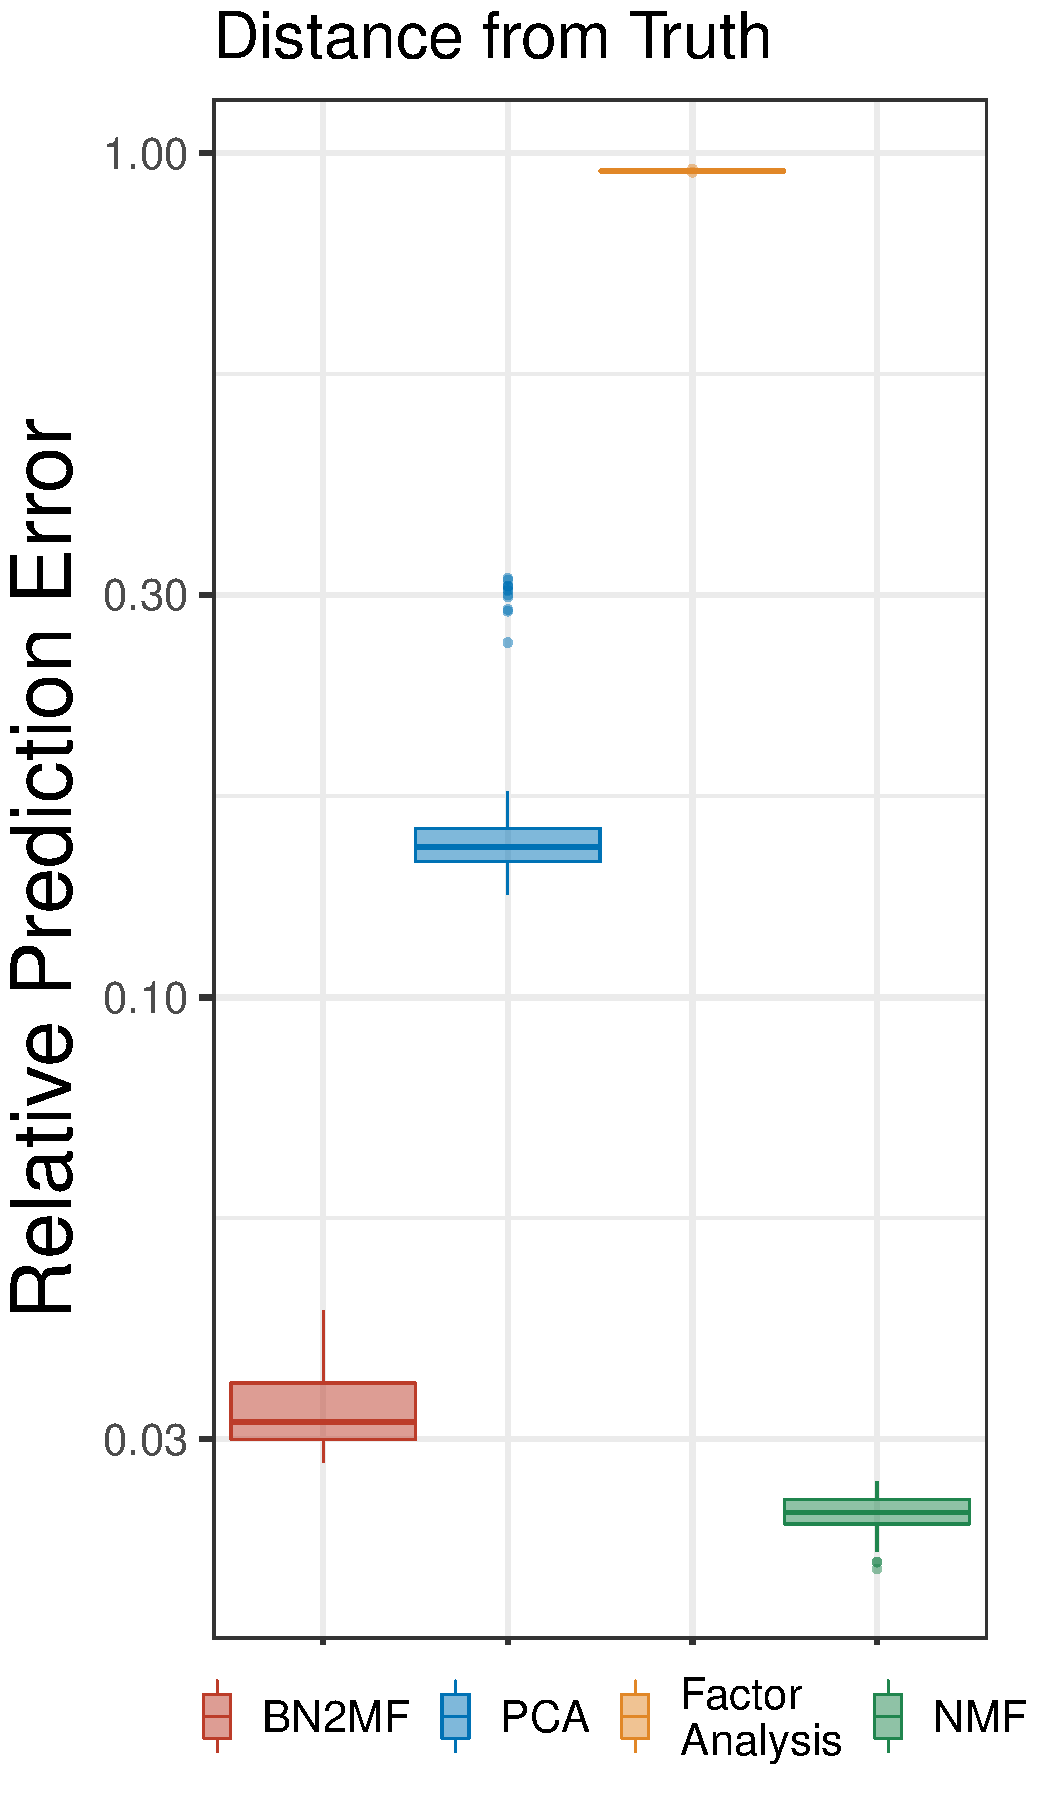
\includegraphics[scale = 0.2]{figures/prime_error.pdf}}
\column{.33\textwidth} 
{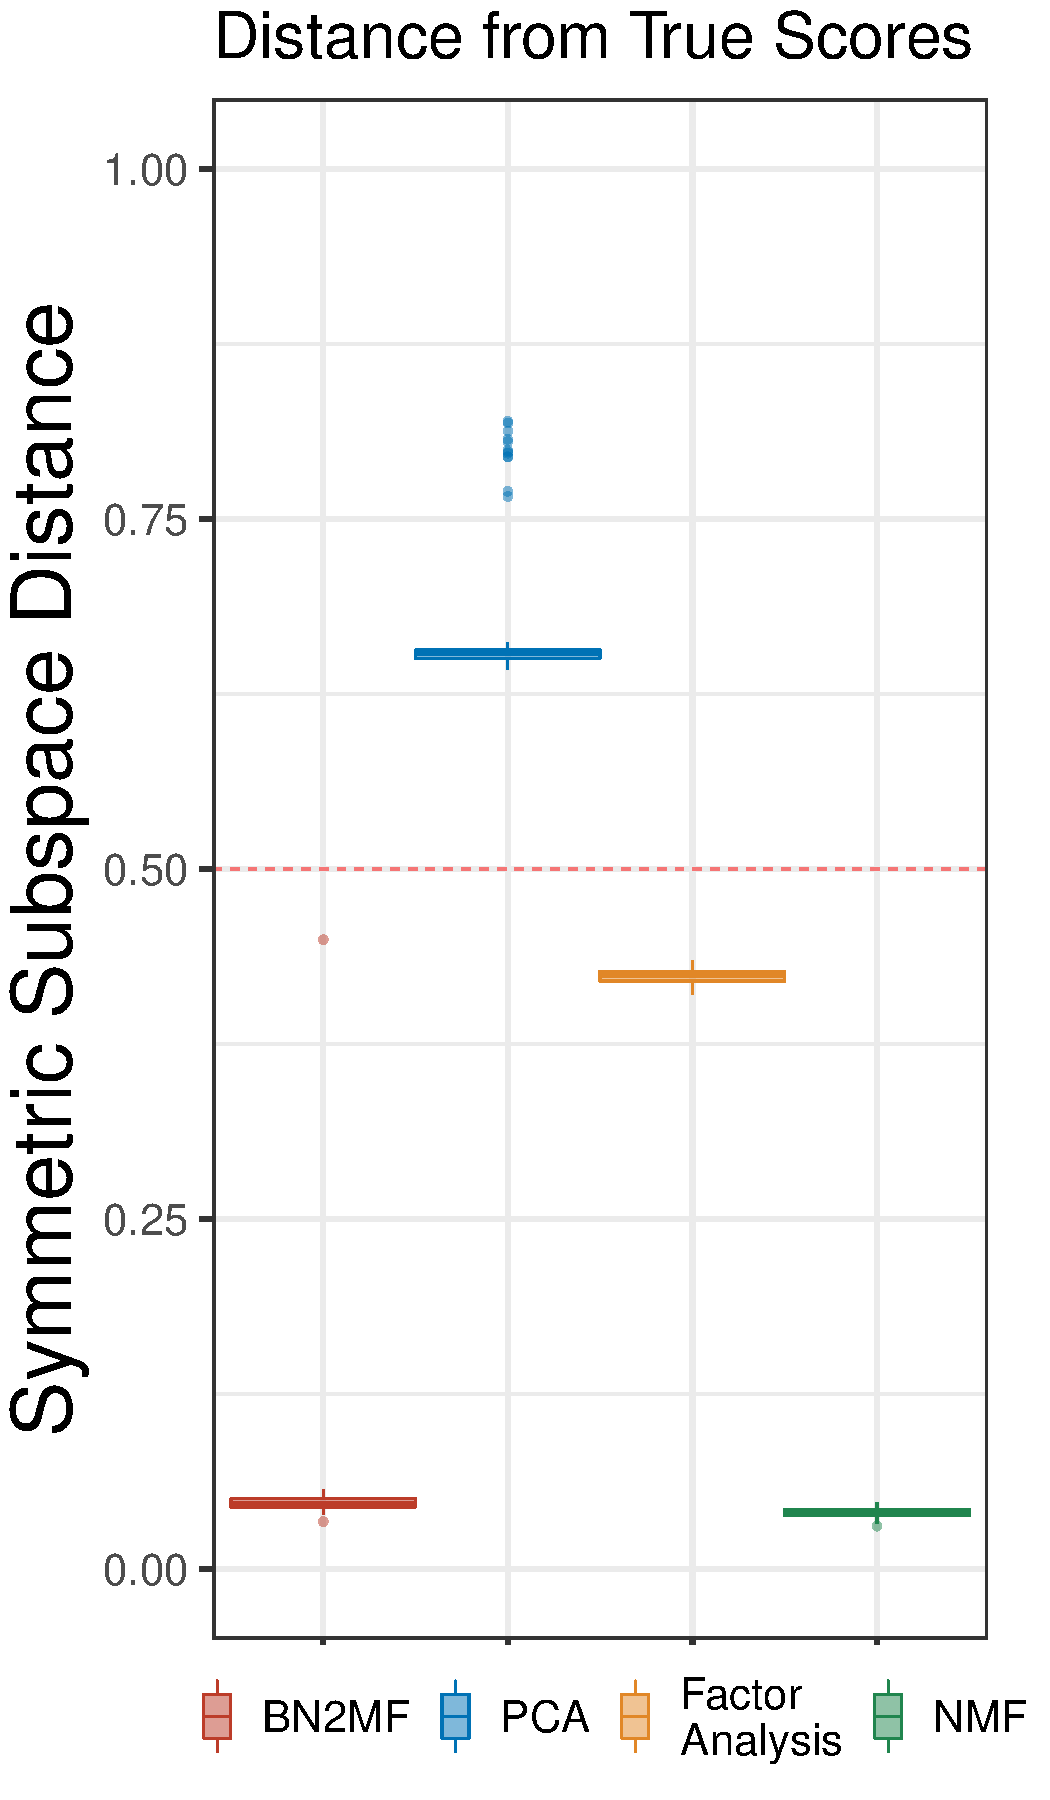
\includegraphics[scale = 0.2]{figures/prime_score.pdf}}
\column{.33\textwidth}
{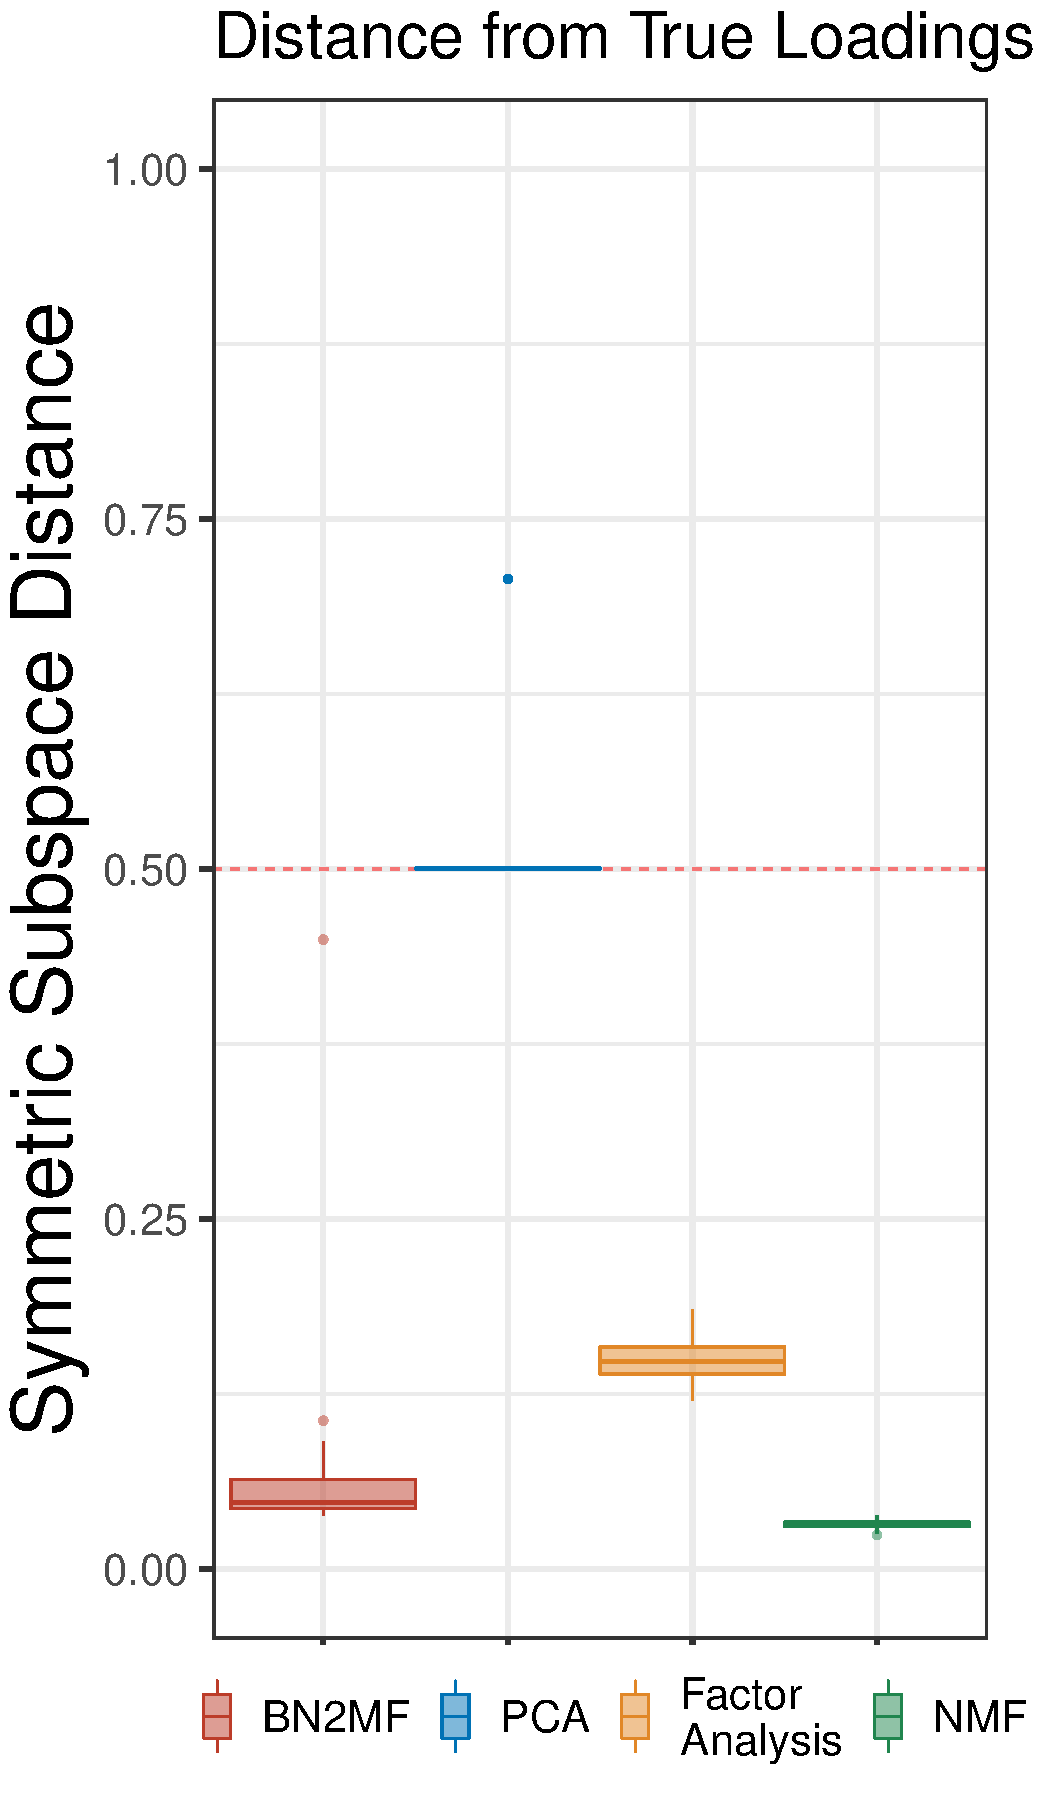
\includegraphics[scale = 0.2]{figures/prime_load.pdf}}
\end{columns}

}

\frame{
\frametitle{Conclusion}
\begin{itemize}
	\item Increased interpretability due to:
	\begin{itemize}
	\item Parts-based (additive) {\color{matbluedark}\textbf{non-negative}} representation of multi-pollutant mixtures
    \item Absence of orthogonality constraint on loadings and scores
	\end{itemize}
	\item[\checkmark] Non-parametric prior on $k$ helps with model selection
	\item[\checkmark] Bayesian framework allows uncertainty propagation
	\item Application to real environmental data can identify sensible patterns
       	\end{itemize}
}
